\item
\begin{align}
\begin{split}
\myvec{\sqrt{2}& \sqrt{3} }\vec{x}&=0
\\
\myvec{\sqrt{3}& \sqrt{8} }\vec{x}&=0
\end{split}
\end{align}
The above equations can be expressed as the matrix equation
\begin{align}
\myvec{\sqrt{2} & \sqrt {3}\\\sqrt{3} & \sqrt{8}} \vec{x} = \myvec{0\\0}
\end{align}
%
The augmented matrix for the above equation is row reduced as follows
\begin{align}
\myvec{\sqrt{2} & \sqrt{3}& 0\\\sqrt {3}& \sqrt{8}& 0} 
\xleftrightarrow {R_2\leftarrow R_2-\frac{\sqrt{3}}{\sqrt{2}}R_1}\myvec{\sqrt{2}& \sqrt{3}& 0\\0 & \frac{1}{\sqrt{2}}& 0}
\\ 
\end{align}%
As left part is converted into identity matrix the intersection vector is\myvec{0\\0} as can be seen in Fig.     \ref{linform/2/10/ef/fig:intersecting lines.}
%
\begin{figure}[ht!]
    \centering
    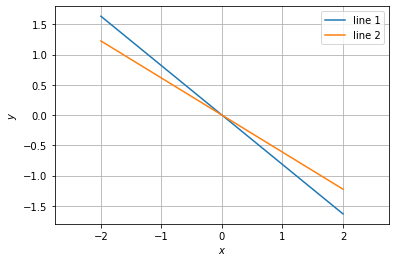
\includegraphics[width=\columnwidth]{solutions/su2021/2/10/ef/Figure2(1).png}
    \caption{intersecting lines}
    \label{linform/2/10/ef/fig:intersecting lines.}
\end{figure} 
\item \begin{align}
\begin{split}
\myvec{\frac{3}{2} & -\frac{5}{3} }\vec{x}&=-2
\\
\myvec{\frac{1}{3} & \frac{1}{2}}\vec{x}&=\frac {13}{6}
\end{split}
\end{align}
The above equations can be expressed as the matrix equation
\begin{align}
\myvec{\frac{3}{2} & -\frac {5}{3}\\\frac{1}{3} & \frac{1}{2}} \vec{x} = \myvec{-2\\\frac{13}{6}}
\end{align}
%
The augmented matrix for the above equation is row reduced as follows\begin{align}
\myvec{\frac{3}{2} & -\frac{5}{3} & -2\\\frac{1}{3} &\frac{1}{2} & \frac{13}{6}}
\xleftrightarrow {R_1\leftarrow 6R_1},\xleftrightarrow {R_2 \leftarrow 6R_2}\myvec{9 & -10 & -12 \\2 & 3 & 13}
\\
%\myvec{9 & -10 & -12\\2 & 3 & 13}
\xleftrightarrow {R_1\leftarrow R_1- 4R_2}\myvec{1 & -22 & -64\\2 & 3 & 13}
\\
%\myvec{1 & -22 & -64\\2 & 3 & 13 }
\xleftrightarrow {R_2\leftarrow R_2-2R_1}\myvec{1 & -22 & -64 \\0 & 47& 141}
\\
%\myvec{1 & -22 & -64\\0 & 47 & 141 }
\xleftrightarrow {R_2\leftarrow R_2/47}\myvec{1 & -22 & -64 \\0 & 1 & 3}
\\
%\myvec {1 & -22 & -64\\0 & 1 & 3}
\xleftrightarrow {R_1 \leftarrow R_1+22R_2}\myvec {1 & 0 & 2\\0 & 1 & 3}
\end{align}
%
As left part is converted into identity matrix the intersection vector is \myvec{2\\3} as can be seen
in Fig.     \ref{linform/2/10/ef/fig: intersecting lines.}


\begin{figure}[!ht]
    \centering
   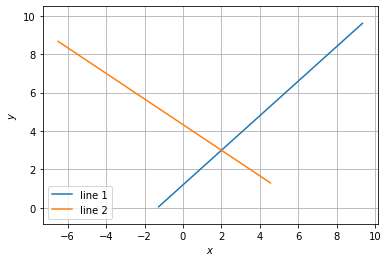
\includegraphics[width=\columnwidth]{solutions/su2021/2/10/ef/Figure2(2).png}
    \caption{intersecting lines}
    \label{linform/2/10/ef/fig: intersecting lines.}
\end{figure}    
\end{enumerate}


